
\documentclass[11pt,a4paper,oneside,english,spanish]{TesisUNI}

\usepackage[natbibapa]{apacite} %Agregar formato de citación APA
\bibliographystyle{apacite}
\setlength{\bibsep}{5pt plus 0.3ex} %Espaciamiento en la bibliografía
\setcounter{secnumdepth}{3} % Numera los subsubsecciones
\usepackage[T1]{fontenc}
\usepackage[spanish, es-tabla]{babel} %% reemplaza "cuadro" por "tabla"
\decimalpoint  %Cambia coma por punto
\usepackage{mathptmx}
\usepackage{layouts} %Saber ancho de hoja.
\usepackage{fontspec}
\usepackage{amssymb}
\usepackage{graphicx}
\usepackage{changepage} %Agregar identación
\setmainfont{Arial}
\usepackage{setspace}
\usepackage[left=4 cm,right=3 cm,top=3 cm,bottom=3.5 cm]{geometry}
\usepackage{fancyhdr} %Encabezado y Pie de página (1)
\pagestyle{fancy} %Encabezado y Pie de página (2)
\usepackage{lipsum} %Crear texto RAMDOM
\renewcommand{\labelitemi}{$\bullet$} %Circulos para viñetas
\usepackage{titlesec} %Titulos de SECCIONES
\usepackage{tocloft} %Titulos de ÍNDICES
\usepackage[colorlinks=true,linkcolor=negro,citecolor = negro]{hyperref}
\usepackage[mathbf=sym]{unicode-math} % Mantener fuentes matemáticas
\makeatletter  %Comando para REDUCIR ERRORES
\usepackage{multirow} % Agregar TABLAS 
\usepackage{array} % Dar formato a las TABLAS
\usepackage{subcaption} % Insertar SubImagenes
\usepackage{tikz} % Diagrama de Flujo
\usetikzlibrary{calc,positioning,shapes.geometric,shapes.symbols,shapes.misc}

% Insertar formas para diagramas de flujo
\tikzstyle{startstop} = [rectangle, rounded corners, minimum width=3cm, minimum height=0.5cm,text centered, draw=black]
\tikzstyle{io} = [trapezium, trapezium left angle=70, trapezium right angle=110, minimum width=3cm, minimum height=0.5cm, text centered, text width=3cm, draw=black]
\tikzstyle{process} = [rectangle, minimum width=3cm, minimum height=0.5cm, text centered, text width=4cm, draw=black]
\tikzstyle{decision} = [diamond, minimum width=3cm, minimum height=0.5cm, text centered, draw=black]
\tikzstyle{loop} = [chamfered rectangle,chamfered rectangle xsep=2cm,draw=black]
\tikzstyle{arrow} = [->,>=stealth]
\tikzstyle{line}=[draw]

\usepackage{listings}
\usepackage{color}

%New colors defined below
\definecolor{codegreen}{rgb}{0,0.6,0}
\definecolor{codegray}{rgb}{0.5,0.5,0.5}
\definecolor{codepurple}{rgb}{0.2,0,1}
\definecolor{codeRojo}{rgb}{0.7,0,0.3}
\definecolor{backcolour}{rgb}{1.0, 1.0, 1.0}

%Code listing style named "mystyle"
\lstdefinestyle{mystyle}{
  backgroundcolor=\color{backcolour},  
  commentstyle=\color{codegreen},
  keywordstyle=\color{codeRojo},
  numberstyle=\tiny\color{codegray},
  stringstyle=\color{codepurple},
  basicstyle=\footnotesize,
  breakatwhitespace=false,         
  breaklines=true,                 
  captionpos=b,                    
  keepspaces=true,                 
  numbers=left,                    
  numbersep=5pt,                  
  showspaces=false,                
  showstringspaces=false,
  showtabs=false,                  
  tabsize=2
}

%"mystyle" code listing set
\lstset{style=mystyle}

\newenvironment{MyFont}{\fontfamily{ugm}\selectfont}{\par}

\usepackage{changepage} %Agregar espacio a Listing



% Centrado del título del ÍNDICE / LISTA DE FIGURAS / LISTA DE CUADROS

\renewcommand{\cfttoctitlefont}{\hfill \normalfont\normalsize\bfseries}
\renewcommand{\cftaftertoctitle}{\hfill}

\renewcommand{\cftlottitlefont}{\hfill\normalfont\normalsize\bfseries}
\renewcommand{\cftafterlottitle}{\hfill}

\renewcommand{\cftloftitlefont}{\hfill\normalfont\normalsize\bfseries}
\renewcommand{\cftafterloftitle}{\hfill}


% Formato de los CAPÍTULOS, SECCIONES Y SUBSECCIONES
\titleformat{\chapter}[block]{\normalfont\normalsize\bfseries}{CAPÍTULO \thechapter:}{0.5em}{\normalsize}
\titlespacing*{\chapter}{0pt}{-10 pt}{5pt}

\titleformat{\section}[block]{\normalfont\normalsize}{\thesection}{0.5em}{\normalsize}
\titlespacing*{\section}{0pt}{10 pt}{5 pt}

\titleformat{\subsection}[block]{\normalfont\normalsize}{\thesubsection}{0.5em}{\normalsize}
\titlespacing*{\subsection}{0pt}{10 pt}{5 pt}

\titleformat{\subsubsection}[block]{\normalfont\normalsize}{\thesubsubsection}{0.5em}{\normalsize}
\titlespacing*{\subsubsection}{0pt}{10 pt}{5 pt}


% Espaciado entre PÁRRAFOS y SANGRÍA
\setlength{\parskip}{5 pt}
\setlength{\parindent}{0cm}


% Dar formato a las TABLAS
\newcolumntype{M}[1]{>{\centering\arraybackslash}m{#1}}
\newcolumntype{L}[1]{>{\raggedright\arraybackslash}m{#1}}
\newcolumntype{R}[1]{>{\raggedleft\arraybackslash}m{#1}}
\newcolumntype{N}{@{}m{0pt}@{}}
\renewcommand{\arraystretch}{1.25}

% Cambiar titulo de bibliografía
\addto\captionsspanish{\renewcommand{\bibname}{\centering REFERENCIAS BIBLIOGRÁFICAS}}


% Posicionamiento vertical de TOC, LOT and LOF

\setlength{\cftbeforelottitleskip}{1pt} 
\renewcommand{\cftafterlottitleskip}{12pt}

\setlength{\cftbeforeloftitleskip}{1pt} 
\renewcommand{\cftafterloftitleskip}{12pt}

\setlength{\cftbeforetoctitleskip}{16pt} 
\renewcommand{\cftaftertoctitleskip}{12 pt}


% Cambiando las etiquetas de las FIGURAS y TABLAS (Caption y autoref)
\addto\captionsspanish{\renewcommand{\figurename}{\footnotesize FIGURA N°}}
\addto\extrasspanish{\def\figureautorefname{ Figura N°}}
 
\addto\captionsspanish{\renewcommand{\tablename}{\footnotesize TABLA N°}}
\addto\extrasspanish{\def\tableautorefname{ Tabla N°}} 


% Espaciamiento dentro del índice

\setlength{\cftbeforechapskip}{2mm}
\renewcommand\cftchapafterpnum{\vskip6pt}
\renewcommand\cftsecafterpnum{\vskip5pt}
\renewcommand\cftsubsecafterpnum{\vskip5pt}


%Agregar la palabra CAPITULO al TOC, FIGURA a LOF y TABLA al LOT

\renewcommand{\cftchappresnum}{CAPÍTULO }
\renewcommand{\cftchapaftersnum}{:}
\renewcommand{\cftchapnumwidth}{7em}

\renewcommand{\cftfigpresnum}{Figura N° }
%\renewcommand{\cftfigaftersnum}{:}
\renewcommand{\cftfignumwidth}{6.85 em}

\renewcommand{\cfttabpresnum}{Tabla N° }
%\renewcommand{\cftfigaftersnum}{:}
\renewcommand{\cfttabnumwidth}{6.5 em}


%Definición de COLORES

\usepackage{xcolor}
\definecolor{granate}{RGB}{113,22,16}
\definecolor{gris}{RGB}{154,153,157}
\definecolor{arena}{RGB}{230,217,170}
\definecolor{azul}{rgb}{0.03, 0.15, 0.4}
\definecolor{negro}{rgb}{0, 0, 0}

%Cambiando a Números Romanos los Capítulos
\renewcommand{\thechapter}{\Roman{chapter}}
\renewcommand{\theequation}{\arabic{chapter}.\arabic{equation}} 
\renewcommand{\thesection}{\arabic{chapter}.\arabic{section}}  
\renewcommand{\thetable}{\arabic{chapter}.\arabic{table}}  
\renewcommand{\thefigure}{\arabic{chapter}.\arabic{figure}}



%Escribir los INFORMACIÓN PERSONAL Y DEL TRABAJO

%Autor para PIE DE PÁGINA (Respetar mayusculas y minisculas)
\author{Nombre1 Nombre2 Apellido1 Apellido2}

%Autor para CARÁTULA (Siempre en mayuscula y sin saltos de linea)
\authorcaratula{NOMBRE1 NOMBRE2 APELLIDO1 APELLIDO2}

%Título en para el PIE DE PÁGINA (Agregar salto de línea de ser necesario)
\title{Xxxxxxxxxxx Título de la Tesis Xxxxxxxxxxx}

%Título para CARÁTULA (Siempre en mayuscula y sin saltos de linea)
\titlecaratula{XXXXXXXXXXXX TÍTULO DE LA TESIS XXXXXXXXXXXXXX}

%Nombre de la FACULTAD (Siempre en mayuscula)
\facultad{FACULTAD DE INGENIERÍA CIVIL}

%Para obtener el título profesional de ... (Siempre en mayuscula)
\grado{INGENIERO CIVIL}

%Asesor para CARÁTULA (Siempre en mayuscula y sin saltos de linea)
\asesor{DR. NOMBRE DEL ASESOR}

%AÑO para CARÁTULA
\yyearr{2021}



\begin{document}
	\nocite{*}
	
	\renewcommand{\BOthers}[1]{et al.\hbox{}} %Agregar et al.
	\onehalfspacing 	% Interlineado 1.5
	\noindent			% Sin sangría
		
	%Parte INCIAL DE LA TESIS
	
	\frontmatter 
		
	\begin{titlepage}
	
	\begin{center}
		\vspace*{2 mm}
		{\LARGE \textbf{UNIVERSIDAD NACIONAL DE INGENIERÍA}}\\
		\vspace{5 mm}
		{\LARGE \textbf{\@facultad}}\\
		\vspace{6.5 mm}
		\begin{figure}[h]
			\centering 
			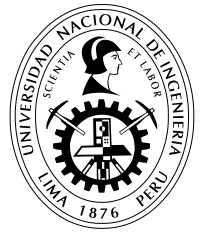
\includegraphics[scale=1]{E_IMAGENES/0_Caratula/UNI_LOGO1.pdf}
		\end{figure}
		\vspace{1 mm}	
		{\Large \textbf{TESIS} }\\
		\vspace{5 mm}
		
		\onehalfspacing  % Espaciamiento 1.5
		{\Large \textbf{``{\@titlecaratula}''} }\\
		
		\singlespacing  % Fin del espaciamiento 1.5
		
		\vspace{5 mm}	
		{\large \textbf{PARA OBTENER EL TÍTULO PROFESIONAL DE {\@grado} } }\\
		\vspace{10 mm}
		{\large \textbf{ELABORADO POR:} }\\
		\vspace{5 mm}	
		{\large \textbf{\@authorcaratula} }\\
		\vspace{10 mm}
		{\large \textbf{ASESOR:} }\\
		\vspace{5 mm}	
		{\large \textbf{\@asesor} }\\
		\vspace{10 mm}	
		{\large \textbf{LIMA - PERÚ} }\\
		\vspace{5 mm}	
		{\large \textbf{\@yyearr} }\\

	\end{center}

\end{titlepage}
	
	\begin{permisos}

	\onehalfspacing  % Espaciamiento 1.5
	
	© 2021, Universidad Nacional de Ingeniería. Todos los derechos reservados \\
	\textbf{``El autor autoriza a la UNI a reproducir la tesis en su totalidad o en parte, con fines estrictamente académicos.''} \\
	Apellido1 Apellido2, Nombre1 Nombre2 \\
	CoreoXXXXX@uni.pe \\
	988654321  
	
	\singlespacing  % Fin del espaciamiento 1.5
	
\end{permisos}


	%\begin{dedication}

Aquí va la dedicatoria\\
a tus padres, hermanos, amigos, etc.

\end{dedication}
	
	%\begin{agradecimientos}
\vspace{50 mm}
\normalsize\textbf{\centerline {AGRADECIMIENTOS}} \newline

\lipsum[17]

\lipsum[11]


\end{agradecimientos}
	
	
	%Cambiar nombre y crear ÍNDICE
	\singlespacing 
	\renewcommand\contentsname{\centering ÍNDICE }
	\tableofcontents	
	\onehalfspacing
	

	\cleardoublepage\phantomsection\addcontentsline{toc}{chapter}{\bf RESUMEN}
\chapter*{\centerline {RESUMEN}}
\markboth{RESUMEN}{}

El objetivo del presente trabajo consiste en el desarrollo de un sistema capaz 
de pronósticar la evolución de tormentas a corto plazo en el territorio peruano.


		
	
	%Cambiar nombre, crear ÍNDICE DE FIGURAS Y TABLAS
	
	\renewcommand\listfigurename{\centering LISTA DE FIGURAS}
	\renewcommand\listtablename{\centering LISTA DE TABLAS}

	\newpage
	%\cleardoublepage\phantomsection\addcontentsline{toc}{chapter}{\listtablename}
	{\normalsize\listoftables}

	\newpage
	%\cleardoublepage\phantomsection\addcontentsline{toc}{chapter}{\listfigurename}
	{\normalsize\listoffigures}
	
	%\cleardoublepage\phantomsection\addcontentsline{toc}{chapter}{LISTA DE SÍMBOLOS Y SIGLAS}	
\chapter*{\centerline {LISTA DE SÍMBOLOS Y SIGLAS}}
\markboth{LISTA DE SÍMBOLOS Y SIGLAS}{}
%---
	\section*{\textbf{\underline{SÍMBOLOS}}}

\begin{tabular}{L{0.5 cm}p{0.025 cm}p{12.5 cm}}
$\alpha$           & : & Razón entre la rigidez postfluencia y la   rigidez elástica \\
$A$                & : & Área de la sección transversal de la viga                                                  \\
$\beta$            & : & Porcentaje de amortiguamiento crítico de la superestructura                                \\
$\beta_{a}$        & : & Fracción de amortiguamiento crítico del AMS                                                \\
$\beta_{M}$        & : & Amortiguamiento efectivo de la edificación aislada                                         \\
$B_{M}$            & : & Factor de reducción asociado al amortiguamiento efectivo   $\beta_{M}$                     \\
$c_{a}$            & : & Amortiguamiento del AMS                                                                     
\end{tabular}






	\newpage
	\section*{\textbf{\underline{SIGLAS}}}

\begin{tabular}{L{1.0 cm}p{0.025 cm}p{11.7 cm}}
ADAS    & : & Added damping and stiffness                                                    \\
AMS     & : & Amortiguador de masa sintonizada                                               \\
AS      & : & Aislador sísmico                                                               \\
ASCE    & : & American society of civil engineers                                            
\end{tabular}\\




 
 
	%Parte CENTRAL DE LA TESIS
	
	\mainmatter 

	% INTRODUCCIÓN
	\chapter{INTRODUCCIÓN}
\markboth{CAPÍTULO \thechapter: INTRODUCCIÓN}{}
	\section{GENERALIDADES}

\lipsum[5]
	\input{2_CAPITULO1/Secciones/2_Descripción del problema.tex}
	\section{Objetivos}
\subsection{Objetivo General}

\lipsum[2]
	
\subsection{Objetivos Específicos}
\begin{itemize}
\item Objetivo específico 1.

\item Objetivo específico 2.

\item Objetivo específico 3.

\end{itemize}





	
	\input{2_CAPITULO1/Secciones/4_Hipótesis.tex}
	\input{2_CAPITULO1/Secciones/5_Metodología.tex}
	



	
	% FUNDAMENTO TEÓRICO Y CONCEPTUAL
	\chapter{MARCO TEÓRICO}
\markboth{CAPÍTULO \thechapter: MARCO TEÓRICO}{}

\lipsum[23]

	\section{Marco Conceptual}

\subsection{Nowcasting}
El pronóstico a corto plazo, conocido como nowcasting fue definido por la
\cite{wmo2017} como el pronóstico con detalles locales, por cualquier método, 
durante un período que va desde el presente hasta 6 horas, incluida una 
descripción detallada del tiempo presente.


\subsection{Geostationary Lightning Mapper}
\cite{GOODMAN201334} definió a el Mapeador de Rayos Geoestacionario (Geostationary Lightning Mapper, GLM) es un
instrumento a bordo del Satélite Geoestacionario Operacional Ambiental 
Geostationary Operational Environmental Satellite, GOES) que mapea actividad de 
rayos continuamente durante el día y noche sobre las Américas y regiones 
oceánicas adyacentes. Conceptualmente, el GLM es un detector de eventos de alta 
velocidad que opera en el espectro infrarojo cercano.



	\section{Marco Tecnológico}

\subsection{Aprendizaje automático}

Según \cite{mitchell1997machine}, el aprendizaje automático (Machine Learning) 
es el estudio de algoritmos que son capaces de mejorar su desempeño en tareas 
específicas por medio del uso de datos.

\subsection{Redes Neuronales Artificiales}

Las redes neuronales artificiales son un modelo compuesto por múltiples capas 
interconectadas de manera similar a las conexiones de neuronas en el cerebro 
humano. Las diferentes arquitecturas de redes neuronales les dan el potencial 
de ser aproximadores universales de funciones \cite{braspenning1995artificial}. 
% Quizá incluir imagenes del simil entre redes neuronales y el cerebro

\subsection{Aprendizaje profundo}

Las técnicas de aprendizaje automático adolecen de un problema fundamental. 
Requieren de dominio considerable del área de aplicación para extraer 
características de los datos y poder transformarlos en una representación 
adecuada para que el modelo pueda reconocer patrones. \cite{LeCun2015} definen
los métodos de aprendizaje profundo (Deep Learning) como métodos que permiten a 
las máquinas descubrir representaciones significativas en conjuntos de datos 
sin procesar.
% Incluir imagenes de un perceptron multicapas


\subsection{Redes Neuronales Convolucionales}

Las redes neuronales convolucionales (Convolutional Neural Networks, CNN) son 
una clase de red neuronal artificial inspiradas por procesos biológicos en los 
que las neuronas responden a estímulos en una región restringida del campo 
visual, denominado campo receptivo (Fukushima, \citeyear{Fukushima1980}). 
\cite{Ciresan2011FlexibleHP} popularizaron su uso al demostrar que la 
aceleración por hardware podía reducir el tiempo de procesamiento en un factor 
de 60. En ese mismo año, usaron dicha implementación para ganar un concurso de 
reconocimiento de imagenes, despertando más interés en la comunidad de visión 
por computador.
% Incluir imagenes de la operación de convolución
% Hablar sobre los parámetros


\subsection{Redes Neuronales Recurrentes}

Las redes neuronales recurrentes (Recurrent Neural Networks, RNN) son una clase 
de red neuronal artificial que permite modelar comportamiento secuencial a lo 
largo de una dimensión (usualmente temporal). Las RNN utilizan un estado interno 
denominado memoria para poder procesar una secuencia de longitud variable de 
entradas \cite{Abiodun2018}.
% Incluir imagenes sobre el tratamiento de secuencias
% Hablar sobre distintos tipos de RNN




	
	\section{Marco Institucional}

El presente trabajo se desarrolla en conjunto con el Servicio Nacional de 
Meteorología e Hidrología del Perú (SENAMHI) para apoyar uno de sus procesos 
misionales.

\subsection{Servicio Nacional de Meteorología e Hidrología del Perú}

El SENAMHI es un organismo público adscrito al Ministerio del Ambiente (MINAM). 
Tiene como misión generar y proveer información y conocimiento meteorológico, 
hidrológico y climático para la sociedad peruana de manera oportuna y 
confiable, contribuyendo de esta manera a la reducción de los impactos 
negativos producidos por los fenómenos naturales de origen hidrometeorológico.

\begin{figure}[H]
  \centering
  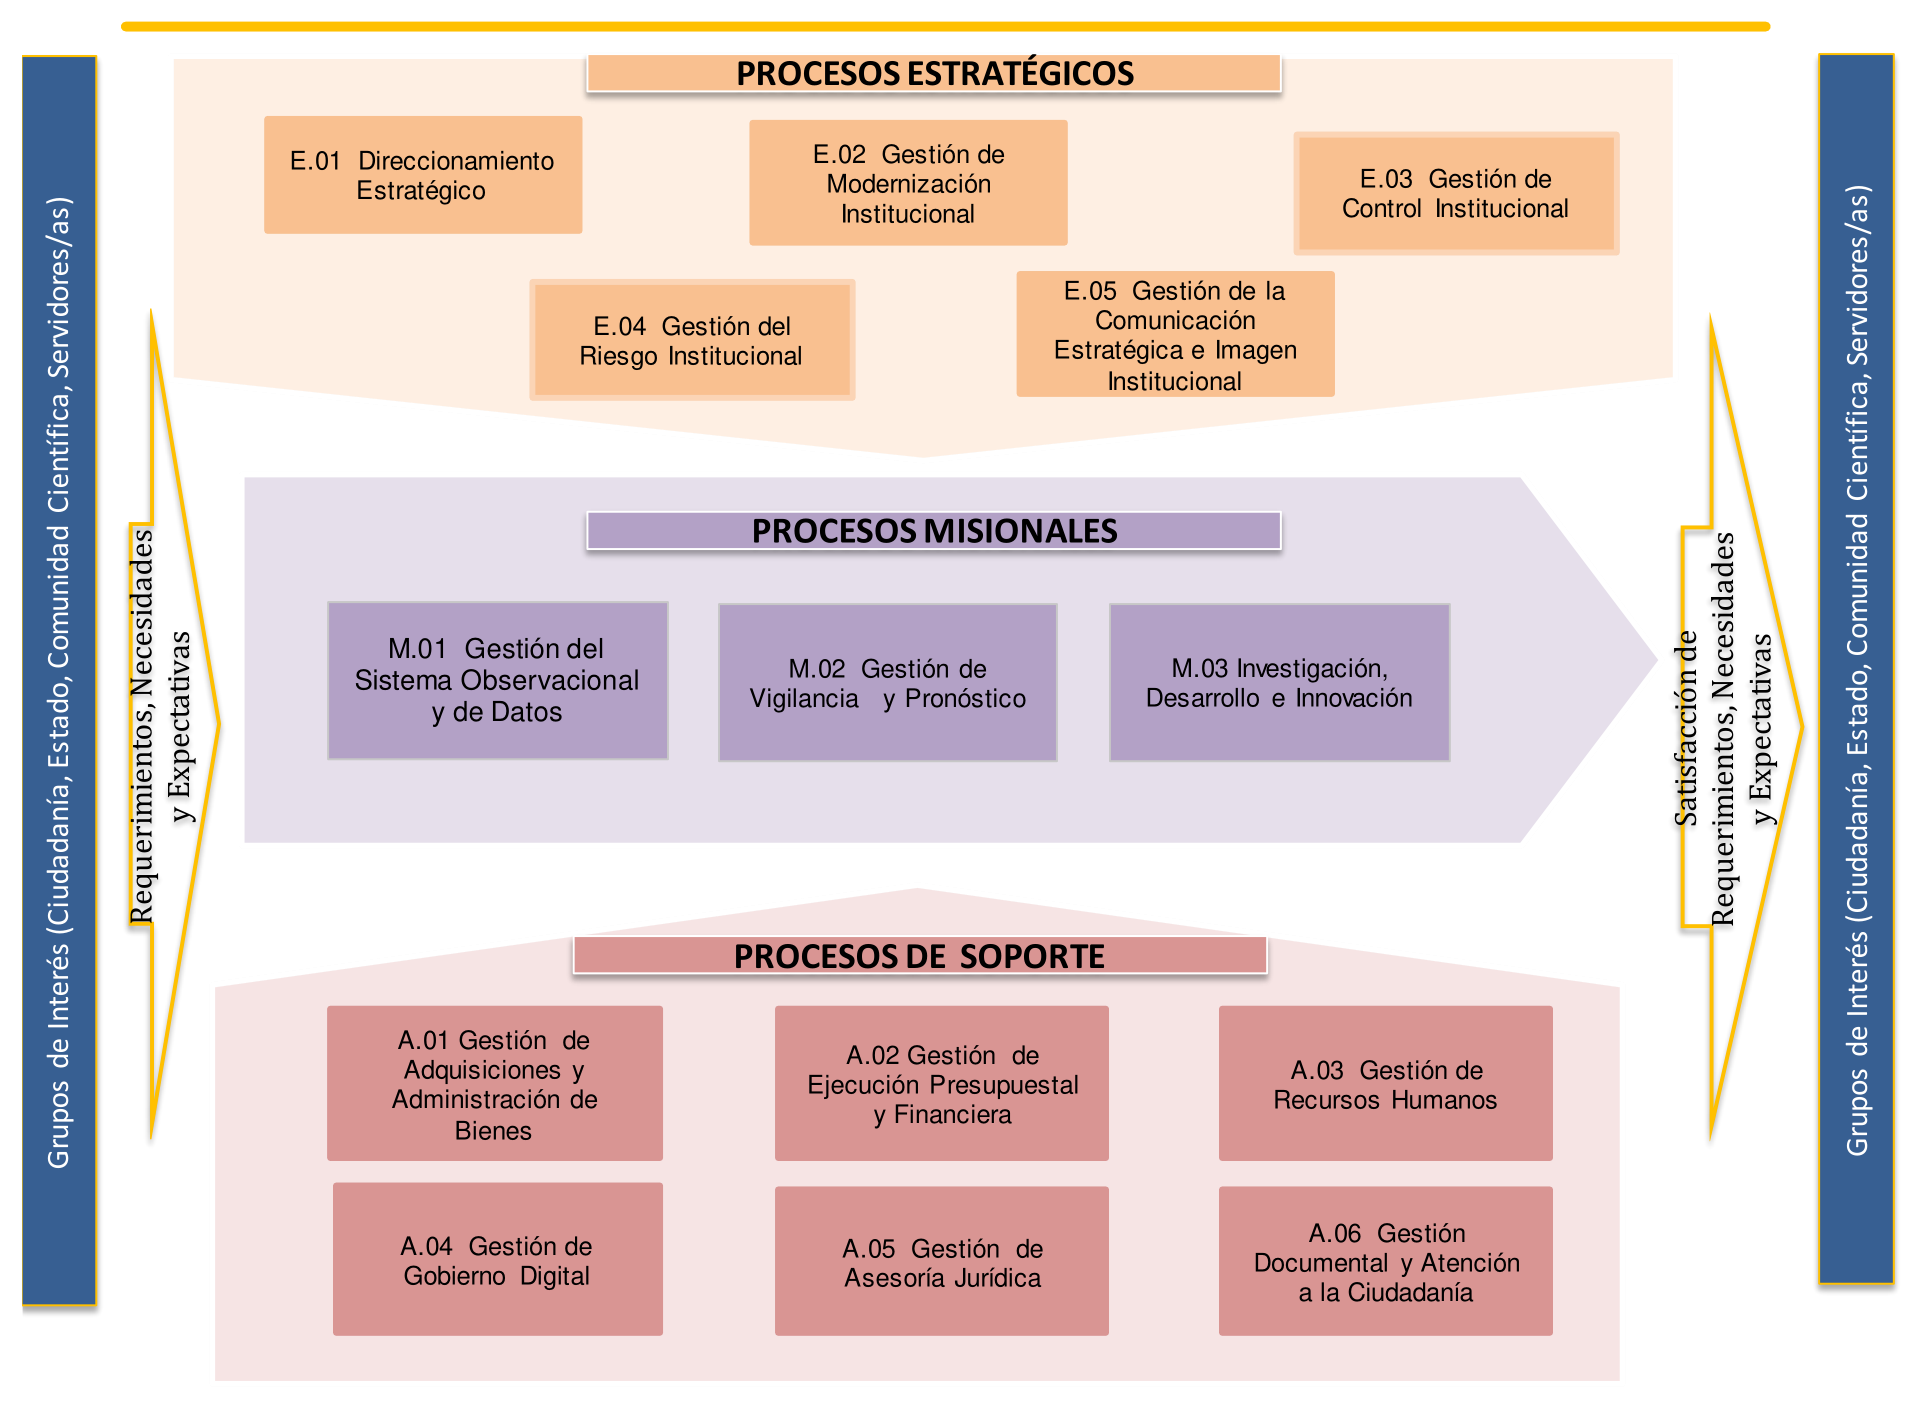
\includegraphics[height=8cm]{E_IMAGENES/2_MarcoTeorico/mapro}
  \caption{
    Mapa de Procesos del SENAMHI.\\
    Fuente: Manual de Procesos y Procedimientos 2020.
  }
  \label{fig:mapro}
\end{figure}

Según \cite{senamhi2020rof} entre sus funciones se encuentra ``Organizar, normar 
y promover un sistema de vigilancia del medio ambiente atmosférico del país, a 
fin de prevenir los peligros de la contaminación ambiental''. Esta función se 
materializa en el proceso misional 02 ``Gestión de Vigilancia y Pronóstico'' del 
Mapa de Procesos que se observa en la figura \ref{fig:mapro}.

\begin{figure}[H]
  \centering
  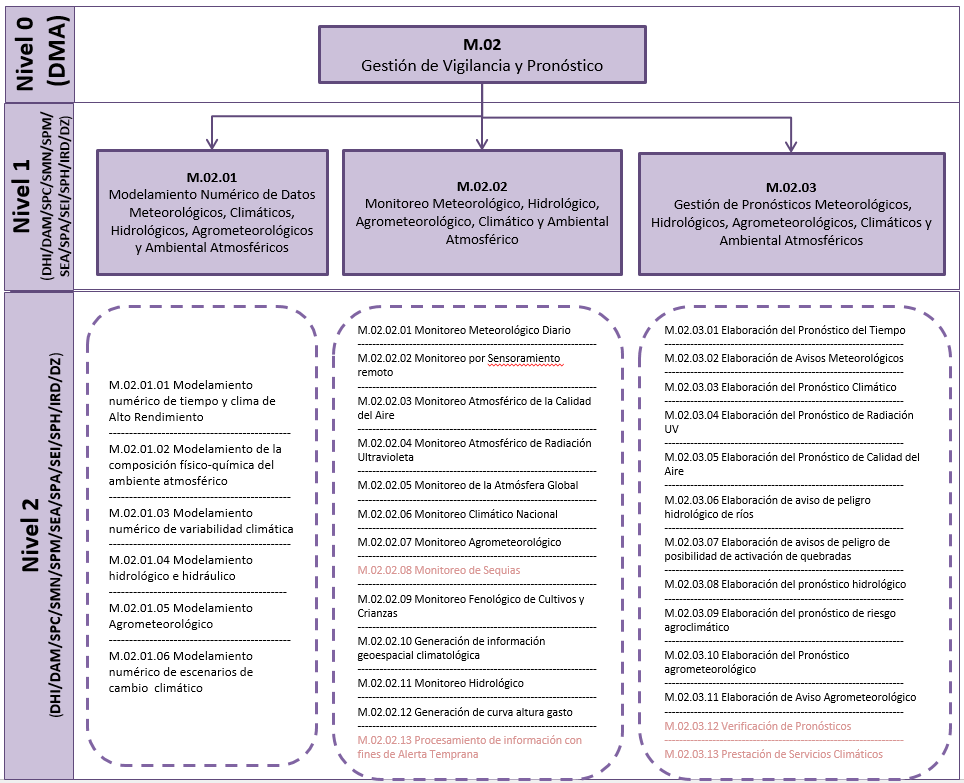
\includegraphics[height=8cm]{E_IMAGENES/2_MarcoTeorico/PM02}
  \caption{
    Proceso misional 02: Gestión de vigilancia y pronóstico\\
    Fuente: Manual de Procesos y Procedimientos 2020.
  }
  \label{fig:pm02}
\end{figure}

El proceso M.02.03, ``Gestión de Pronósticos Meteorológicos, Hidrológicos, 
Agrometeorológicos, Climáticos y Ambiental Atmosféricos'', que se observa en la 
figura \ref{fig:pm02} comprende entre sus procedimientos la elaboración de 
pronósticos del tiempo y tiene como uno de sus productos el pronóstico a muy 
corto plazo. 

De acuerdo a \cite{senamhi2021govdig}, es parte del Plan de Gobierno Digital del 
SENAMHI la ampliación de funcionalidades del sistema de pronóstico inmediato 
(nowcasting).

	
	\section{Marco Legal y Normativo}

\subsection{Lineamientos para el diseño de sistemas integrados de vigilancia y 
pronóstico hidrometeorológico con fines de alerta temprana}

\cite{senamhi2021lineamientos} indica que los servicios y productos asociados a 
la alerta temprana deben obedecer el principio de subsidiariedad, lo que 
significa que los avisos de peligro a muy corto plazo deben poder ser generados 
por las oficinas desconcentradas del SENAMHI.\newline
La continuidad del servicio requiere además un sistema robusto y resiliente, 
siguiendo el principio de subsidiariedad, la sede central del SENAMHI apoyaría 
a los organos desconcentrados en la generación o entrega de productos en caso 
de que sus capacidades se vean sobrepasadas.

\subsection{Recommendation of the Council on Artificial Intelligence}

De acuerdo con \cite{oecd2019recom} uno de los principios para la 
administración responsable de la inteligencia artificial es la 
\textbf{Robustez, seguridad y protección}:
\begin{itemize}
  \item Los sistemas de IA deben ser robustos y seguros durante todo su ciclo 
  de   vida de tal manera que, en condiciones de uso normal, uso o maluso 
  previsible,   u otras condiciones adversas, funcionen apropiadamente y no 
  planteen un riesgo de seguridad no razonable.
  \item Para este fin, los actores involucrados deben asegurar la trazabilidad, 
  incluso en relación a los conjuntos de datos, procesos y decisiones hechas 
  durante el ciclo de vida del sistema, para habilitar el análisis de los 
  resultados del sistema.
  \item Los actores deberán, basado en sus roles, aplicar un enfoque 
  sistemático de gestión de riesgos a cada fase del ciclo de vida del sistema 
  para atender los riesgos relacionados a sistemas de IA, incluyendo seguridad 
  digital y sesgo.
\end{itemize}


% Lineamientos para el diseño de sistemas integrados de vigilancia y pronóstico hidrometeorológico con fines de alerta temprana
% ENIA Peru

	


	
		
	% CAPÍTULO 3
	\chapter{ESTADO DEL ARTE}
\markboth{CAPÍTULO \thechapter: ESTADO DEL ARTE}{}

\section{Taxonomía}

Se ha desarrollado una cantidad significativa de trabajo en el área de 
pronóstico a muy corto plazo de secuencias espaciotemporales. Dado que 
el pronóstico de tormentas eléctricas está intimamente relacionado con el 
pronóstico de secuencias espaciotemporales este capítulo presentará una 
taxonomía de enfoques de pronóstico de secuencias espaciotemporales a muy 
corto plazo.\newline
La taxonomía presentada en la figura \ref{fig:taxonomia} en forma de árbol, 
dividida en dos ramas principales para las categorías de enfoques utilizados. 
Cada una de estas ramas es dividida en subcategorías de enfoques utilizados. 
Cada enfoque utilizado es subidividido en métodos utilizados.

\begin{figure}[H]
  \centering
  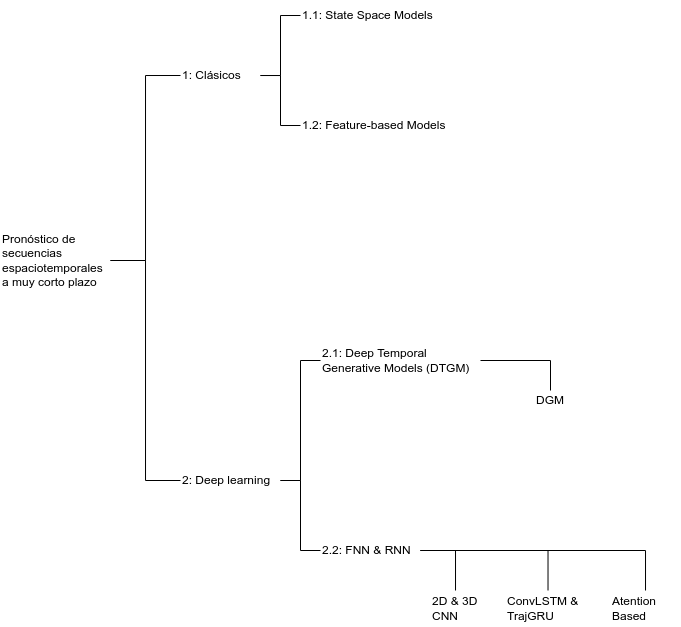
\includegraphics[width=14cm]{./E_IMAGENES/3_EstadoArte/taxonomia}
  \caption{
    Una taxónomía de los enfoques aplicados a la predicción de secuencias 
    espaciotemporales a muy corto plazo. Categorías extraidas de 
    \cite{DBLP:journals/corr/abs-1808-06865}.
  }
  \label{fig:taxonomia}
\end{figure}

El foco del presente trabajo está en el uso de técnicas de deep learning, por 
lo que no se realizaron mayores subdivisiones en los métodos clásicos.

\subsection{Enfoques Clásicos}
Dado que una secuencia espaciotemporal puede ser vista como una secuencia 
multivariada, los métodos diseñados para el pronóstico de series de tiempo 
multivariadas son aplicables a secuencias espaciotemporales.

\subsubsection{State Space Models}
Los Modelos de Espacio de Estados (State Space Models, SSM) analiza a las 
secuencias desde un punto de vista generativo, donde cada observación $X_t$ se 
asume generada por un estado oculto $H_t$ y esos estados ocultos forman un 
proceso de Markov. Ejemplos notables de este tipo de modelos son los 
Autoregressive Integrated Moving Average Model (ARIMA).

\subsubsection{Feature-based Models}
Los modelos basados en características resuelve el pronóstico de secuencias 
espaciotemporales al entrenar un modelo de regresión basado en características 
diseñadas por humanos.

\subsection{Enfoques Deep Learning}
Los enfoques de deep learning propuestos para el modelamiento de secuencias 
espaciotemporales aprovechan las capacidades de generalización de las redes
neuronales profundas.

\subsubsection{Deep Temporal Generative Models}
Los Modelos Generativos Profundos son modelos estadísticos que aprenden 
distribuciones de probabilidad de los datos y permiten facil generación de 
muestras de sus distribuciones aprendidas.

\begin{itemize}
  \item \textbf{DGM}: \cite{Ravuri2021} propuso el uso de Redes Generativas 
  Adversariales (Generative Adversarial Network, GAN) para modelar datos de 
  precipitación de radares meteorológicos en Reino Unido. El modelo propuesto 
  busca resolver el problema de pronósticos difuminados aprovechando la 
  capacidad de las GAN para generar pronósticos feasibles a cualquier plazo a 
  futuro.
  \begin{figure}[H]
    \centering
    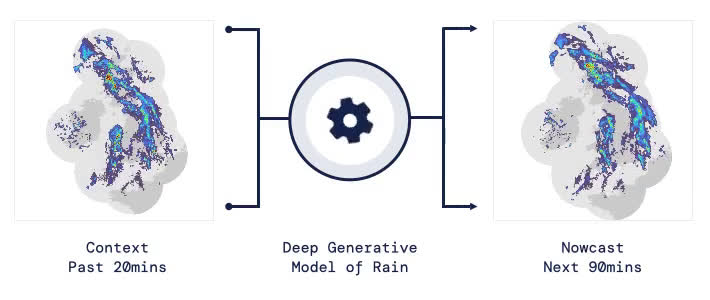
\includegraphics[width=8cm]{E_IMAGENES/3_EstadoArte/dgmr_1}
    \caption{
      Modelo de pronóstico de lluvia a muy corto plazo utilizando Redes 
      Generativas Adversariales. Fuente: \cite{Ravuri2021}
    }
    \label{fig:dgmr_modelo}
  \end{figure}
\end{itemize}

\subsubsection{FNN \& RNN}
\begin{itemize}
  \item \textbf{2D \& 3D CNN}: \cite{Cintineo2020} propuso el uso de Redes 
  Neuronales Convolucionales para pronósticar la probabilidad de convección 
  intensa. Su trabajo fue complementado con la explicabilidad de los 
  pronósticos, descubriendo los factores más significativos en el resultado del 
  modelo.
  \begin{figure}[H]
    \centering
    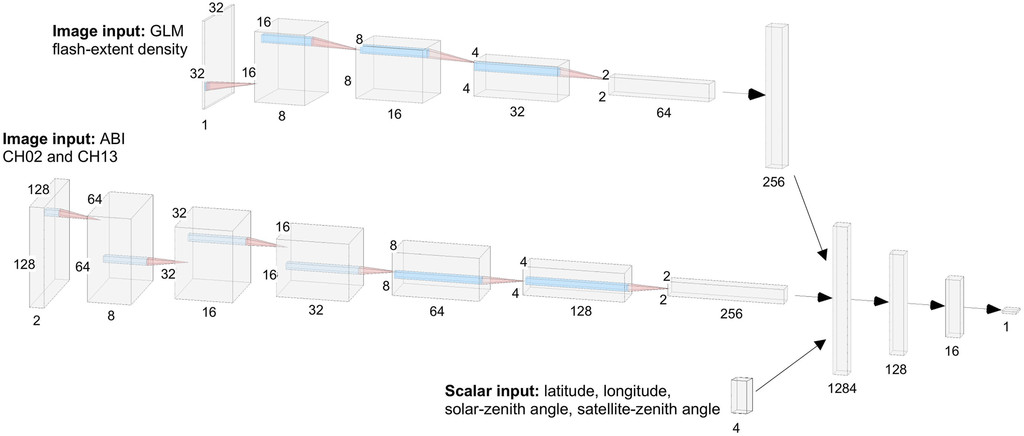
\includegraphics[width=10cm]{E_IMAGENES/3_EstadoArte/cintineo_1}
    \caption{
      Arquitectura de redes neuronales convolucionales para el pronóstico de 
      convección intensa. Fuente: \cite{Cintineo2020}.
    }
    \label{fig:cintineo}
  \end{figure}
  \cite{Chang2018} propuso el uso de datos topográficos para mejorar el 
  desempeño un modelo de pronóstico de precipitación, obteniendo mejor 
  desempeño que el modelo inicial, sin embargo, la proporción de falsa alarma 
  también se incrementó. Este artículo propone la incorporación de información 
  topográfica usando un bloque de convolución y max pooling como se observa en 
  la figura \ref{fig:chang}
  \begin{figure}[H]
    \centering
    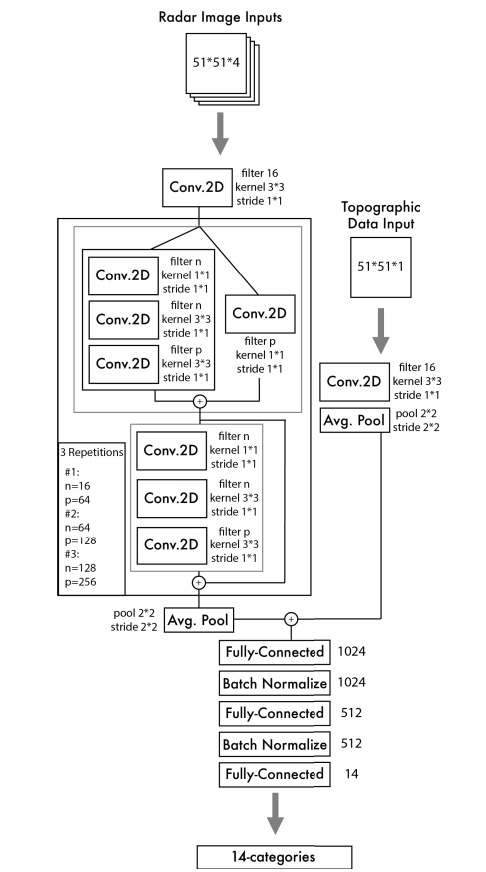
\includegraphics[width=8cm]{E_IMAGENES/3_EstadoArte/chang_1}
    \caption{
      Arquitectura de redes neuronales convolucionales que incorpora datos 
      topográficos. Fuente: \cite{Chang2018}.
    }
    \label{fig:chang}
  \end{figure}

  \item \textbf{ConvLSTM \& TrajGRU}: \cite{DBLP:journals/corr/ShiCWYWW15} 
  propuso una arquitectura de redes neuronales que combina la capacidad de 
  capturar correlación espacial de las CNN y la capacidad de capturar 
  correlación temporal de las LSTM, la denominó ConvLSTM. Las ConvLSTM utilizan 
  un estado oculto multidimensional para poder capturar información espacial y 
  actualizan sus estados por medio de la operación de convolución. 
  \begin{figure}[H]
    \centering
    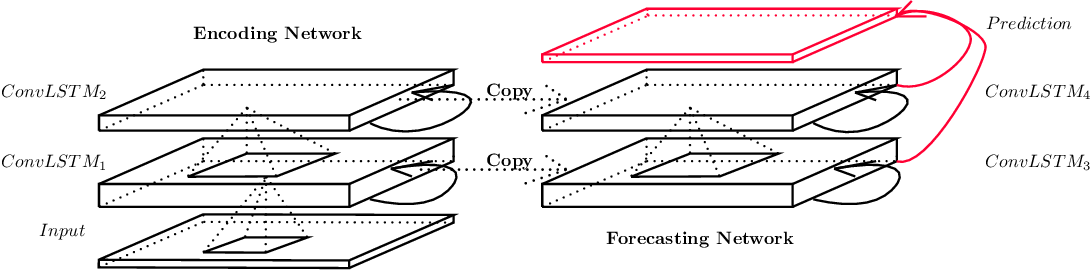
\includegraphics[width=8cm]{E_IMAGENES/3_EstadoArte/convlstm}
    \caption{
      Arquitectura de red neuronal convolucional LSTM para el pronóstico 
      inmediato de precipitación. Fuente: \cite{DBLP:journals/corr/ShiCWYWW15}.
    }
    \label{fig:convlstm}
  \end{figure}
  \cite{DBLP:journals/corr/ShiGL0YWW17} evaluó el desempeño de distintos 
  modelos de pronóstico inmediato para precipitación y propuso una nueva 
  arquitectura que resolvería el problema de la falta de sensibilidad a la 
  rotación de la arquitectura ConvLSTM, la denominó TrajGRU.
  \begin{figure}[H]
    \centering
    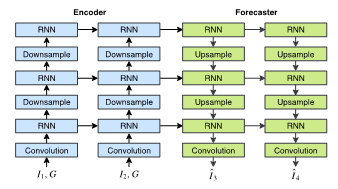
\includegraphics[width=8cm]{E_IMAGENES/3_EstadoArte/trajgru}
    \caption{
      Arquitectura de red neuronal Trajectory GRU para el pronóstico 
      inmediato de precipitación. Fuente: \cite{DBLP:journals/corr/ShiGL0YWW17}.
    }
    \label{fig:trajgru}
  \end{figure}

  \item \textbf{Atention based}: \cite{DBLP:journals/corr/abs-2003-12140} 
  propuso una arquitectura que utilice el mecanismo de atención para poder 
  capturar correlaciones temporales a largo plazo, la denominó MetNet. Su 
  arquitectura presentada en la figura \ref{fig:metnet} entrega como salida 
  distribuciones de probabilidad de precipitiación con un desempeño que supera 
  a los modelos actualmente empleados. El modelo cuenta con 225M parámetros 
  entrenables, por lo que su entrenamiento y despliegue requiere de un enorme 
  poder computacional.
  \begin{figure}[H]
    \centering
    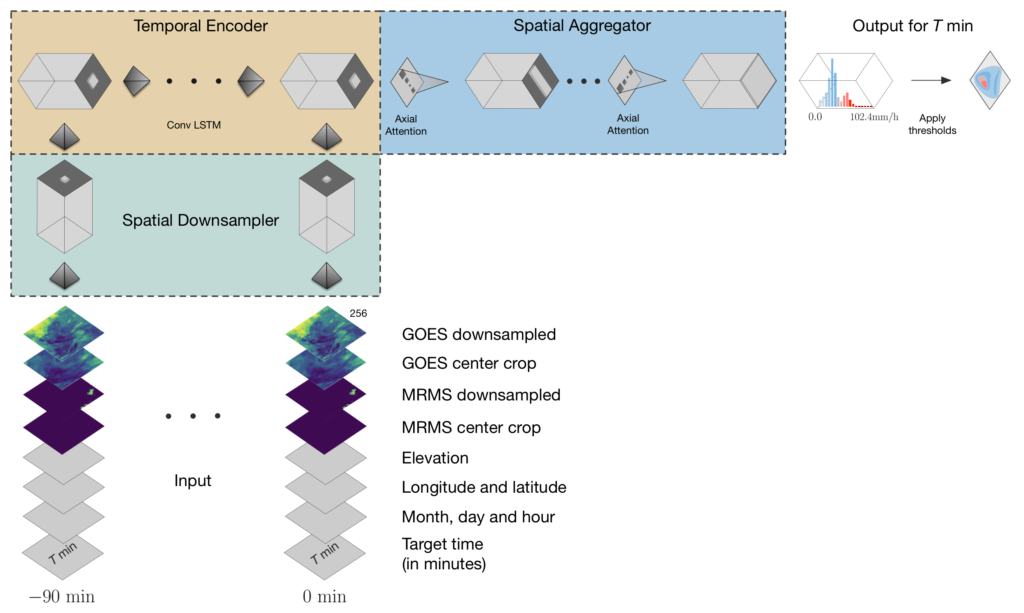
\includegraphics[width=12cm]{E_IMAGENES/3_EstadoArte/metnet}
    \caption{
      Arquitectura de red neuronal MetNet. Fuente: 
      \cite{DBLP:journals/corr/abs-2003-12140}.
    }
    \label{fig:metnet}
  \end{figure}

\end{itemize}




\section{Benchmarking}

Se realizará una comparación entre los métodos descritos en el estado del arte. 
Se utilizarán criterios con pesos asignados siguiendo el Proceso Analítico 
Jerarquico (Analytical Hierarchical Process, AHP).
		
\subsection{Criterios}

\begin{itemize}
  \item \textbf{C1. Complejidad de entrenamiento:} Es el tiempo que 
  el modelo necesita para generalizar los datos, estimado en base a la 
  complejidad del modelo por usando el númeo de parámetros como indicador.
  \item \textbf{C2. Desempeño a muy corto plazo:} Es el desempeño definido por 
  las métricas de evaluación pertinentes.
  \item \textbf{C3. Explicabilidad:} Es la capacidad de reconocer los factores 
  que determinan el resultado del modelo. Es importante para poder obtener un 
  mayor conocimiento del fenómeno de estudio.
  \item \textbf{C4. Replicabilidad:} Es la disponibilidad de recursos que 
  soporten el desarrollo de un tipo de método y su uso con los datos 
  disponibles.
\end{itemize}

\subsection{Cálculo de pesos}
Se utilizó la escala de Saaty (ver tabla \ref{tab:escala_saaty}), para poder 
determinar la importancia relativa de los criterios respecto a ellos mismos.

\begin{table}[H]
  \centering
  \caption{Escala de Saaty}
  \begin{tabular}{ll}
  \textbf{Intensidad} & \textbf{Definición}    \\ \hline
  1                   & Igual importancia      \\
  3                   & Moderada importancia   \\
  5                   & Importancia fuerte     \\
  7                   & Importancia muy fuerte \\
  9                   & Importancia extrema    \\
  2, 4, 6, 7          & Valores intermedios   
  \end{tabular}
  \label{tab:escala_saaty}
\end{table}


\begin{table}[H]
  \centering
  \caption{Matriz de comparaciones pareadas.}
  \begin{tabular}{l|cccc}
  \hline
  \textbf{}     & \multicolumn{1}{l}{C1} & \multicolumn{1}{l}{C2} & \multicolumn{1}{l}{C3} & \multicolumn{1}{l}{C4} \\ \hline
  C1 & 1   & 3   & 5   & 1/5 \\
  C2 & 1/3 & 1   & 3   & 1/3 \\
  C3 & 1/5 & 1/3 & 1   & 3   \\
  C4 & 5   & 3   & 1/3 & 1   \\ \hline
  \textbf{Suma} & 98/15 = 6.53           & 22/3 = 7.33            & 28/3 = 9.33            & 68/15 = 4.53           \\ \hline
  \end{tabular}
  \label{tab:comp_pareadas}
\end{table}

\begin{table}[H]
  \centering
  \caption{Cálculo de los pesos.}
  \begin{tabular}{l|cccc|l}
  \hline
  \textbf{} & \multicolumn{1}{l}{C1} & \multicolumn{1}{l}{C2} & \multicolumn{1}{l}{C3} & \multicolumn{1}{l|}{C4} & \textbf{Peso} \\ \hline
  C1 & 0.153  & 0.409  & 0.536  & 0.0442 & 0.2855 \\
  C2 & 0.0510 & 0.136  & 0.322  & 0.0736 & 0.1457 \\
  C3 & 0.0306 & 0.0455 & 0.107  & 0.662  & 0.2113 \\
  C4 & 0.766  & 0.409  & 0.0357 & 0.221  & 0.358  \\ \hline
  \end{tabular}
  \label{tab:comp_pareadas_norm}
\end{table}

De la tabla \ref{tab:comp_pareadas_norm} obtenemos que el criterio 4 
(Replicabilidad) es el más importante, seguido de Complejidad de entrenamiento, 
Explicabilidad y finalmente el desempeño a corto plazo. Esto se dió debido a 
que el stakeholder valora más una solución funcional que pueda ir mejorando con 
el tiempo a una solución compleja cuya implementación y explicabilidad sea 
baja.

\subsection{Evaluación}
Las alternativas a evaluar son:

\begin{itemize}
  \item \textbf{A1. DGM}
  \item \textbf{A2. 2D \& 3D CNN} 
  \item \textbf{A3. ConvLSTM \& TrajGRU} 
  \item \textbf{A4. Atention Based}
\end{itemize}

\begin{table}[H]
  \centering
  \caption{Evaluación de las alternativas.}
  \begin{tabular}{l|ccccl}
  \hline
  \textbf{}            & \multicolumn{1}{l}{C1}     & \multicolumn{1}{l}{C2}     & \multicolumn{1}{l}{C3}     & \multicolumn{1}{l}{C4}    & Total \\ \hline
  A1 & 0.0833 & 0.324  & 0.0928 & 0.0657  & 0.1141  \\
  A2 & 0.333  & 0.221  & 0.3571 & 0.3947  & 0.3440  \\
  A3 & 0.416  & 0.0567 & 0.4285 & 0.4802  & 0.3894  \\
  A4 & 0.166  & 0.396  & 0.1214 & 0.05921 & 0.15193 \\ \hline
  \textbf{Ponderación} & \multicolumn{1}{l}{0.2855} & \multicolumn{1}{l}{0.1457} & \multicolumn{1}{l}{0.2113} & \multicolumn{1}{l}{0.358} &       \\ \hline
  \end{tabular}
  \label{tab:evaluacion}

\end{table}

\subsection{Decisión}

De acuerdo a los puntajes obtenidos en la tabla \ref{tab:evaluacion}, se elige 
la alternativa 3 (ConvLSTM \& TrajGRU).

	




		


		
	% CAPÍTULO 4
	\chapter{APORTE DE LA TESIS}
\markboth{CAPÍTULO \thechapter: APORTE DE LA TESIS}{}

\section{Caja negra}
Una caja negra es un sistema que puede ser definido en terminos de sus entradas 
y salidas, sin conocimiento de su funcionamiento interno. Su implementación es 
opaca (negra). Se describirán los elementos del artefacto propuesto a 
continuación.

\textbf{Entradas:}
\begin{itemize}
  \item Flash Extend Density (FED) del satélite GOES-16.
\end{itemize}

\textbf{Habilitadores:}
\begin{itemize}
  \item Servidores de procesamiento.
  \item Sistema de alerta temprana.
\end{itemize}

\textbf{Restricciones:}
\begin{itemize}
  \item Tiempo de respuesta del satélite GOES-16.
  \item Tormentas eléctricas atípicas.
\end{itemize}


\textbf{Salidas:}
\begin{itemize}
  \item Probabilidad de ocurrencia de densidad de rayos (rayos/km$^2$).
\end{itemize}

\begin{figure}[H]
  \centering
  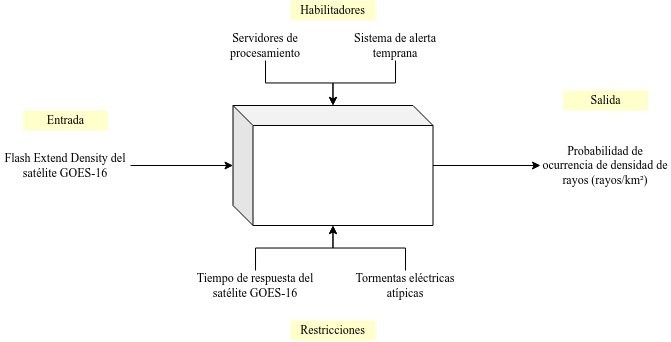
\includegraphics[width=14cm]{E_IMAGENES/4_Aporte/CajaNegra.png}
  \caption{
    Caja negra.
  }
  \label{fig:cajanegra}
\end{figure}

		
	
	%Parte FINAL DE LA TESIS
	
	\backmatter

	% CONCLUSIONES
	\cleardoublepage\phantomsection\addcontentsline{toc}{chapter}{\bf CONCLUSIONES}
\chapter*{\centerline {CONCLUSIONES}}
\markboth{CONCLUSIONES}{}
%--
%\begin{enumerate}

%\item Nam dui ligula, fringilla a, euismod sodales, sollicitudin vel, wisi.  Morbiauctor lorem non justo. Nam lacus libero, pretium at, lobortis vitae, ultricies et,tellus. Donec aliquet, tortor sed accumsan bibendum, erat ligula aliquet magna,vitae ornare odio metus a mi.

%\item Nam dui ligula, fringilla a, euismod sodales, sollicitudin vel, wisi.  Morbiauctor lorem non justo. Nam lacus libero, pretium at, lobortis vitae, ultricies et,tellus. Donec aliquet, tortor sed accumsan bibendum, erat ligula aliquet magna,vitae ornare odio metus a mi.

%\item Nam dui ligula, fringilla a, euismod sodales, sollicitudin vel, wisi.  Morbiauctor lorem non justo. Nam lacus libero, pretium at, lobortis vitae, ultricies et,tellus. Donec aliquet, tortor sed accumsan bibendum, erat ligula aliquet magna,vitae ornare odio metus a mi.


%\end{enumerate}

	
	% RECOMENDACIONES	
	\cleardoublepage\phantomsection\addcontentsline{toc}{chapter}{\bf RECOMENDACIONES}
\chapter*{\centerline {RECOMENDACIONES}}
\markboth{RECOMENDACIONES}{}
%
\begin{enumerate}
\item Nam dui ligula, fringilla a, euismod sodales, sollicitudin vel, wisi.  Morbiauctor lorem non justo. Nam lacus libero, pretium at, lobortis vitae, ultricies et,tellus. Donec aliquet, tortor sed accumsan bibendum, erat ligula aliquet magna,vitae ornare odio metus a mi.

\item Nam dui ligula, fringilla a, euismod sodales, sollicitudin vel, wisi.  Morbiauctor lorem non justo. Nam lacus libero, pretium at, lobortis vitae, ultricies et,tellus. Donec aliquet, tortor sed accumsan bibendum, erat ligula aliquet magna,vitae ornare odio metus a mi.

\item Nam dui ligula, fringilla a, euismod sodales, sollicitudin vel, wisi.  Morbiauctor lorem non justo. Nam lacus libero, pretium at, lobortis vitae, ultricies et,tellus. Donec aliquet, tortor sed accumsan bibendum, erat ligula aliquet magna,vitae ornare odio metus a mi.


\end{enumerate}
	
	% REFERENCIAS BIBLIOGRÁFICAS
	\cleardoublepage\phantomsection\addcontentsline{toc}{chapter}{\bf REFERENCIAS BIBLIOGRÁFICAS}
\begingroup
\titleformat*{\chapter}{\normalfont\bfseries\normalsize\centering}
\bibliography{3_3_BIBLIOGRAFIA/library}
\endgroup


	
	% ANEXOS	
	\cleardoublepage\phantomsection\addcontentsline{toc}{chapter}{\bf ANEXOS}
\chapter*{\centerline {ANEXOS}}
\markboth{ANEXOS}{}
%---

% Definir númeración y citación para Listing 

\renewcommand{\lstlistingname}{ \footnotesize Código A \hspace{-1.75mm}}% Cambiar el nombre a Algoritmo
\renewcommand*{\thelstlisting}{.\arabic{lstlisting}} 
\def\lstlistingautorefname{Código A\hspace{-0.75mm}}

% Redefinir númeración y citación para Figuras
\renewcommand\thefigure{.\arabic{figure}}  
\setcounter{figure}{0} 
\renewcommand\figurename{\footnotesize FIGURA B \hspace{-1.6mm}}
\def\figureautorefname{Figura B \hspace{-2mm}}


	\section*{ANEXO A: CÓDIGOS EN PYTHON}
\phantomsection
\addcontentsline{toc}{section}{ANEXO A: CÓDIGOS EN PYTHON}
A continuación se presentan los códigos desarrollados en \textit{Python}. En este sentido, el \autoref{Algoritmo1} muestra el algoritmo usado para edificaciones con aislamiento de base con comportamiento bilineal. El \autoref{Algoritmo2} muestra las funciones usadas por los algoritmos anteriormente mencionados.

\vspace*{2mm}


	\subsection*{Respuesta Sísmica de una Edificación con AS}
%\phantomsubsection
\addcontentsline{toc}{subsection}{Respuesta Sísmica de una Edificación con AS}

\begin{MyFont}
\begin{adjustwidth}{4.8mm}{}
\begin{lstlisting}[language=Python, caption= {\footnotesize Edificación con aislamiento sísmico bilineal}, mathescape=true,label={Algoritmo1}]
# REPUESTA SÍSMICA DE UNA EDIFICACIÓN DE n NIVELES CON AS
import Funciones_KS as fun
import numpy as np
from scipy  import linalg as LA
import copy

# PROPIEDADES DINÁMICAS
# Parámetros dinámicos de la Superestructura
n=3                 # N° de Pisos
gdl=n+1             # GDL = N° de Pisos+1
Tnf=0.3             # Periodo base fija, [s]
$\xi$=5           			 # Amortiguamiento, [%]
$\lambda$=(gdl-1)/gdl 			 # Relación de masas

# Parámetros dinámicos de la interfaz de aislamiento
r=0.1               # Razón de rigideces Kp/Ke
Q=105          		  # Fuerza característica normalizada, [cm/s^2]
K2=30         		  # Rigidez postfluencia normalizada, [1/s^2]

# LECTURA DEL REGISTRO SÍSMICO
ug=np.genfromtxt("./Sismo_Lima66NS.txt")  #[cm/s^2]
$\Delta$t=0.002; N=len(ug)
t=[i*$\Delta$t for i in range(N)]

\end{lstlisting}
\end{adjustwidth}
\end{MyFont}

	
	\subsection*{Funciones}
%\phantomsubsection
\addcontentsline{toc}{subsection}{Funciones}

\begin{MyFont}
\begin{adjustwidth}{4.8mm}{}
\begin{lstlisting}[language=Python, caption={\footnotesize Funciones-KS}, mathescape=true,label={Algoritmo2}]
import numpy as np
from scipy  import linalg as LA
import copy

# FUNCIÓN EIGEN
def eigen(Tsf=1,n=5):
    Z=np.identity(n); ke=(4*n/Tsf)**2; k=np.zeros(n)
    for i in range(n):
        if i==0:
            k[i]=2*ke
        else:
            k[i]=ke
    K=tridiag(k,n); M=np.identity(n)
    vp,$\varphi$p=LA.eigh(K,M); $\varphi$p=$\varphi$p.T; FP=[]; MP=[] 
    for i in range(n):
        FP.append(sum($\varphi$p[i].T@M))
    for i in range(n):
        MP.append((sum($\varphi$p[i].T@M))**2)
    T=2*np.pi/(vp)**0.5; MMP=MP/sum(MP)
    return T,$\varphi$p,FP,MMP

\end{lstlisting}
\end{adjustwidth}
\end{MyFont}

	\newpage

	\section*{ANEXO B: HISTÉRESIS DE LOS DISPOSITIVOS DE CONTROL}
\phantomsection
\addcontentsline{toc}{section}{ANEXO B: HISTÉRESIS DE LOS DISPOSITIVOS DE CONTROL}

\lipsum[10]

	\subsection*{Edificio Principal del Aeropuerto Jorge Chavez}
%\phantomsubsection
\addcontentsline{toc}{subsection}{Edificio Principal del Aeropuerto Jorge Chavez}

La \autoref{Anexo_1} muestra las histéresis de uno de los dos los DFV instalados en el eje 5-5 del primer nivel del edificio pincipal del aeropuerto Jorge Chavez. Asimismo, la \autoref{Anexo_2} presenta la histéresis de uno de los tres DH-SLB colocado en el eje 5-5 del primer nivel de la misma edificación.


	\begin{figure}[!h]
	\centering
	\includegraphics[scale=1]{E_IMAGENES/Anexos/Anexo_1.pdf}
	\vspace{-8 mm}
	\caption[]{\centering\footnotesize Histéresis del DFV del edificio del aeropuerto Jorge Chavez.}
	\label{Anexo_1}
	\end{figure}	


	\begin{figure}[!h]
	\centering
	\includegraphics[scale=1]{E_IMAGENES/Anexos/Anexo_2.pdf}
	\vspace{-8 mm}
	\caption[]{\centering\footnotesize Histéresis del DH-SLB del edificio del aeropuerto Jorge Chavez.}
	\label{Anexo_2}
	\end{figure}	





	
\end{document}